\subsection{Уравнения Лагранжа}

\begin{figure}
\begin{minipage}[t]{0.3\textwidth}
    \centering
    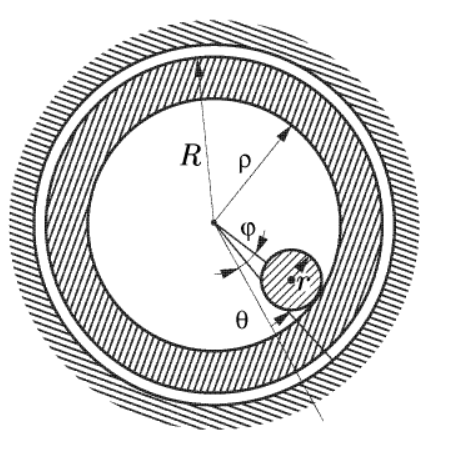
\includegraphics[width=0.9\textwidth]{figures/12.46.png}
    \caption{К задаче 12.46}
    \label{t12n46}
\end{minipage}
\hfill
\begin{minipage}[t]{0.3\textwidth}
    \centering
    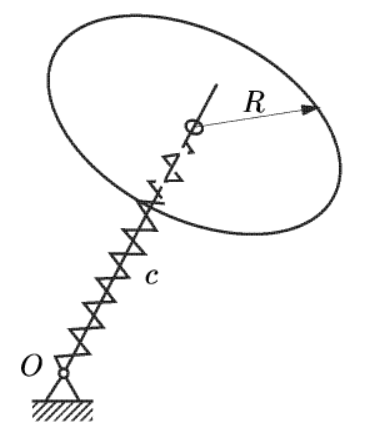
\includegraphics[width=0.8\textwidth]{figures/12.59.png}
    \caption{К задаче 12.59}
    \label{t12n59}
\end{minipage}
\hfill
\begin{minipage}[t]{0.3\textwidth}
    \centering
    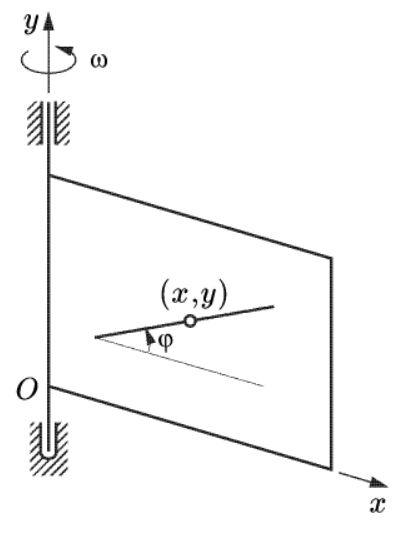
\includegraphics[width=0.8\textwidth]{figures/12.61.png}
    \caption{К задаче 12.61}
    \label{t12n61}
\end{minipage}
\end{figure}



\subsubsection*{12.6 (в)}

Проверим, является ли интегрируемой связь 
\begin{equation*}
    \dot{y} - z \dot{x} = 0.
\end{equation*}
В случае интегрируемости связи существовали бы запрещенные положения системы. Покажем же что в действительности мы можем попасть из любой точки в любую. В силу отсутсвия ограничений на $\dot{z}$, мы свободно можем перемещаться вдоль оси $z$ при $\dot{x}, \dot{y} = 0$. Пусть мы оказались в $z = 2$, тогда при движении
\begin{equation*}
    \letus \ \dot{x} \d t = \xi,
    \ \ \dot{y} \d t=  2 \xi, \hspace{0.5cm} \Rightarrow \hspace{0.5cm} 
    (0, 0, 2) \longrightarrow (\xi, 2 \xi, 2).
\end{equation*}
Теперь по $\dot{x}, \dot{y} = 0$ перейдём в $z = 1$, тогда
\begin{equation*}
    \letus \ \dot{x} \d t = -\xi, \ \ \dot{y} \d t = -\xi,
    \hspace{0.5cm} \Rightarrow \hspace{0.5cm} 
    (\xi, 2 \xi, 1) \longrightarrow (0, \xi, 1).
\end{equation*}
Собирая всё вместе,
\begin{equation*}
    (0, 0, 0)
    \overset{\vv{\dot{r}} = (0, 0, \neq 0)}{\longrightarrow} 
    (0, 0, 2)
    \overset{\vv{\dot{r}}dt = (\xi, 2\xi, 2)}{\longrightarrow} 
    (\xi, 2 \xi, 2)
    \overset{\vv{\dot{r}} = (0, 0, \neq 0)}{\longrightarrow} 
    (0, 0, 1)
    \overset{\vv{\dot{r}}dt = (-\xi, -\xi, 1)}{\longrightarrow} 
    (0, \xi, 1)
    \overset{\vv{\dot{r}} = (0, 0, \neq 0)}{\longrightarrow} 
    (0, \xi, 0).
\end{equation*}
Получается допустимы перемещения из $\vc{r}_1$ в $\vc{r}_2$ $\forall \vc{r}_1, \vc{r}_2$, следовательно \textbf{связь не является интегрируемой}.


\subsubsection*{12.12}

Найдём уравнения движения для двух материальных точек, массами $m_1$ и $m_2$, притягивающихся по закону Ньютона. В качестве обобщенных координат выберем $x, y, z$ центра масс системы, расстояние между точками $r$ и углы $\varphi, \theta$, определяющие направление прямой. 

Потенциальная энергия системы $\Pi$ 
\begin{equation*}
    \Pi = - \gamma \frac{m_1 m_2}{r}.
\end{equation*}
Для каждого из тел можем записать расстояние до центра масс и абсолютное положение:
\begin{equation*}
    r_1 = \frac{m_2}{m_1+m_2} r, \hspace{0.5cm} 
    r_2 = \frac{m_1}{m_1+m_2} r,
    \hspace{0.5cm} 
    \left\{\begin{aligned}
        x_1 &= x + r_1 \sin \theta \cos \varphi, \\
        y_1 &= y + r_1 \sin \theta \cos \varphi, \\
        z_1 &= z + r_1 \cos \theta.
    \end{aligned}\right.
    \hspace{0.5cm} 
    \left\{\begin{aligned}
        x_2 &= x + r_2 \sin \theta \cos \varphi, \\
        y_2 &= y + r_2 \sin \theta \cos \varphi, \\
        z_2 &= z + r_2 \cos \theta.
    \end{aligned}\right.
\end{equation*}
Вспомнив, что для сферических координат$(r,  \theta, \varphi)$ метрический тензор $g_{ij} = \diag \left({1}, \ {r^2}, \ {r^2 \sin^2 \theta} \right)$, найдём  квадрат относительной скорости
\begin{equation*}
    v_1^2(r_1) = g_{ij} \dot{q}^i \dot{q}^j = 
    r_1^2 \sin^2 \theta \dot{\varphi}^2 + r_1^2 \dot{\theta}^2 + \dot{r_1}^2 
    \hspace{0.5cm} \Rightarrow \hspace{0.5cm} 
    v_1^2(r_1) = \left(
    \frac{m_2}{m_1+m_2} 
    \right)^2 \cdot v_1^2 (r).
\end{equation*}
Теперь можем записать кинетическую энергию движения ($T_1, T_2$ -- кинетические энергии движения тел относительно центра масс) :
\begin{equation*}
    T_1 + T_2 + \frac{1}{2} (m_1+m_2) \left(\frac{d}{dt} (x, \ y, \ z)\right)^2 =
    \frac{1}{2} \frac{m_1 m_2}{m_1 + m_2} 
    \left(
        r^2 \sin^2 \theta \dot{\varphi}^2 + r^2 \dot{\theta}^2 + \dot{r}^2
    \right) + 
    \frac{1}{2} (m_1+m_2) \left(\dot{x}^2 + \dot{y}^2 + \dot{z}^2\right).
\end{equation*}
И, наконец, лагранжиан системы
\begin{equation}
    L = T - \Pi = \frac{1}{2} \frac{m_1 m_2}{m_1 + m_2} 
    \left(
        r^2 \sin^2 \theta \dot{\varphi}^2 + r^2 \dot{\theta}^2 + \dot{r}^2
    \right) + 
    \frac{1}{2} (m_1+m_2) \left(\dot{x}^2 + \dot{y}^2 + \dot{z}^2\right)
    + \gamma \frac{m_1 m_2}{r}.
\end{equation}
Найдём уравнения движения системы относительно центра масс:
\begin{equation}
    \left\{\begin{aligned}
        \frac{d }{d t} \frac{\partial L}{\partial \dot{\varphi}} - \frac{\partial L}{\partial \varphi} &= 0 \\
        \frac{d }{d t} \frac{\partial L}{\partial \dot{r}} - \frac{\partial L}{\partial r} &= 0 \\
        \frac{d }{d t} \frac{\partial L}{\partial \dot{\theta}} - \frac{\partial L}{\partial \theta} &= 0.
    \end{aligned}\right.
    \hspace{0.5cm} \Rightarrow \hspace{0.5cm} 
    \left\{\begin{aligned}
        \dot{\varphi} \left(
        r  \dot{\theta} \sin (2 \theta) + \dot{r} \dot{\varphi} (1 - \cos 2 \theta)
    \right) 
    + \frac{1}{2} r \ddot{\varphi} \left(
         1 - \cos 2 \theta
    \right) = 0, 
    \\
        \gamma (m_1 + m_2) - r^3
    \left(
        \sin^2 \theta \dot{\varphi}^2 + \dot{\theta}^2
    \right) + r^2 \ddot{r} = 0,
    \\
    2 \dot{\theta} \dot{r} + r \ddot{\theta} - \frac{1}{2} r \sin (2 \theta) \dot{\varphi}^2 = 0.
    \end{aligned}\right.
\end{equation}
И для центра масс:
\begin{equation}
    \ddot{x} = 0, \hspace{0.5cm} 
    \ddot{y} = 0, \hspace{0.5cm} 
    \ddot{z} = 0.
\end{equation}
Что логично, на центр масс не действует никаких сил.

Теперь к интегралам системы. Пусть $\frac{d }{d t} (x_1, y_1, z_1)\T = \vc{v}_1$, аналогично для второго тела. Во-первых сохраняется количество движения системы
($x, \ y, \ z$ не входят явно в $L$), также не входят $t, \ \varphi$, тогда
\begin{equation}
    \left\{\begin{aligned}
        \frac{d }{d t} \frac{\partial L}{\partial x} &= 0 \\
        \frac{d }{d t} \frac{\partial L}{\partial \varphi} &= 0 \\
        L &\neq L(t)
    \end{aligned}\right.    
    \hspace{0.5cm} \Rightarrow \hspace{0.5cm} 
    \left\{\begin{aligned}
        m_1 \vc{v}_1 + m_2 \vc{v}_2 &= \const, \\
        r^2 \dot{\varphi} \sin^2 \theta  &= \const, \\
        E = \Pi + T &= \const.
    \end{aligned}\right.
\end{equation}
Вообще, в силу отсутсвия внешних сил на систему, сохраняется кинетический момент,
\begin{equation}
    \vc{K} = m_1 \vc{r}_1 \times \vc{v}_1 + 
    m_2 \vc{r}_2 \times \vc{v}_2 = \const.
\end{equation}

\subsubsection*{12.29}

Два однородных стержня длины $l$ каждый образую плоский двойной маятник. Составим уравнения движения в форме Лагранжа. 

Выберем начала координат в точке подвеса. Тогда координаты центра масс второго стержня
\begin{equation*}
    \left\{\begin{aligned}
        x_2 &= l \sin \varphi_1 + (l/2) \sin \varphi_2, \\
        y_2 &= l \cos \varphi_1 + (l/2) \cos \varphi_2.
    \end{aligned}\right.
\end{equation*}
Потенциальная энергия системы
\begin{equation*}
    \Pi = -mg \left(\frac{l}{2} \cos \varphi_1 \right) -
    mg \left(
        l \cos \varphi_1 + \frac{l}{2} \cos \varphi_2
    \right).
\end{equation*}
Кинетическая энергия первого стержня
\begin{equation*}
    T_1 = \frac{1}{2} I_1 \dot{\varphi}_1^2 = \frac{l^2 m}{6}  \dot{\varphi}^2.
\end{equation*}
Для второго стержня найдём кинетическую энергию, рассмотрев его вращение относительно центра масс:
\begin{equation*}
    T_2 = \frac{1}{2} m \left( \dot{x}_2^2 + \dot{y}_2^2\right) +
    \frac{1}{2} \frac{m l^2}{12}  \dot{\varphi}_2^2.
\end{equation*}
Лагранжиан системы:
\begin{equation}
    L = T - \Pi 
    =  ml^2 \left[
        \frac{g}{2l} \left( 3 \sin \varphi_1 +  \cos \varphi_2  \right)
        + \frac{1}{2} \cos (\varphi_1 - \varphi_2) \dot{\varphi}_1 \dot{\varphi}_2 + \frac{2}{3}  \dot{\varphi}^2 + \frac{1}{6} \dot{\varphi}_2^2
        \right].
\end{equation}
Тогда уравнения движения системы
\begin{equation}
    \left\{\begin{aligned}
        \frac{d }{d t} \frac{\partial L}{\partial \dot{\varphi_1}} - \frac{\partial L}{\partial \varphi_1} &= 0, \\
        \frac{d }{d t} \frac{\partial L}{\partial \dot{\varphi_2}} - \frac{\partial L}{\partial \varphi_2} &= 0.
    \end{aligned}\right.
    \hspace{0.5cm} \Rightarrow \hspace{0.5cm} 
    \left\{\begin{aligned}
    9 (g/l) \sin \varphi_1 + 3  \sin (\varphi_1 - \varphi_2) \dot{\varphi}^2_2
    + 3 \cos (\varphi_1 - \varphi_2) \ddot{\varphi}_2 + 8  \ddot{\varphi}_1 &= 0, \\
    3 (g/l) \sin \varphi_2 - 3  \sin (\varphi_1 - \varphi_2) \dot{\varphi}_1^2
    + 3 \cos (\varphi_1 - \varphi_2) \ddot{\varphi}_1 + 2  \ddot{\varphi}_2 &= 0.
    \end{aligned}\right.
\end{equation}
\subsubsection*{12.46}

Составим уравнения движения в форме Лагранжа для системы, представленно на рис. \ref{t12n46} Для начала запишем потенциальную энергию системы, как
\begin{equation*}
    \Pi = - (\rho - r) \cos (\varphi  + \theta).
\end{equation*}
Момент инерции полого цилиндра:
\begin{equation*}
    I_1 = \int_\rho^R \sigma r^2 \d V 
    \hspace{0.2cm} 
    \overset{dV = h 2 \pi r \d r}{\longrightarrow} 
    \hspace{0.2cm} 
    I_1 = 2 \pi \sigma h \int_\rho^R r^3 \d r = 
    \frac{1}{2} \left(R^2 - \rho^2  \right) (R^2 + \rho^2) \pi  h \sigma =
    \frac{1}{2} M \left(R^2 + \rho^2\right).
\end{equation*}
Тогда его кинетическая энергия 
\begin{equation*}
    T_1 = \frac{1}{4} M \left(R^2 + \rho^2\right) \dot{\theta}^2.
\end{equation*}
Скорость центра масс сплошного цилиндра:
\begin{equation*}
    v_2 = \dot{\varphi} (\rho  - r).
\end{equation*}
Пусть цилиндр катится с угловой скоростью $\omega$, тогда запишем условие того, что он не проскальзывает
\begin{equation*}
    (\rho - r) \dot{\varphi} = \rho \dot{\theta} + \omega r,
    \hspace{0.5cm} \Rightarrow \hspace{0.5cm} 
    \omega = (\rho - r) \dot{\varphi} - \rho \dot{\theta}.
\end{equation*}
Тогда кинетическая энергия сплошного цилиндра
\begin{equation*}
    T_2 = 
    \frac{1}{2} m \left(
        \dot{\varphi} (\rho - r) \vp
    \right)^2 + 
    \frac{1}{2} \left(\frac{1}{2} m r^2 \right) \omega^2
    .
\end{equation*}
Лагранжиан системы:
\begin{equation}
    L = 
    mg (\rho - r) \cos \varphi +
     m \left(
        \frac{1}{2}  \dot{\varphi}^2 (\rho - r)^2 + 
        \frac{1}{4} \left(
            \dot{\theta} \rho - \dot{\varphi} (\rho - r)
        \right)^2
    \right) + \frac{1}{4} M \left(R^2  + \rho^2\right)\dot{\theta}^2.
\end{equation}
Соответсвенно, уравнения движения системы
\begin{equation}
    \left\{\begin{aligned}
        \frac{d }{d t} \frac{\partial L}{\partial \dot{\varphi}} - \frac{\partial L}{\partial \varphi} &= 0, \\
        \frac{d }{d t} \frac{\partial L}{\partial \dot{\theta}} - \frac{\partial L}{\partial \theta} &= 0.
    \end{aligned}\right.
    \hspace{0.5cm} \Rightarrow \hspace{0.5cm} 
    \left\{\begin{aligned}
    - \ddot{\theta} \rho + 3 \ddot{\varphi} \left(\rho - r\right) + 2 g \sin{\left(\varphi \right)} &= 0, \\
    M \ddot{\theta} \left(R^{2} + \rho^{2}\right) + \rho m \left(\ddot{\theta} \rho - \ddot{\varphi} \left(\rho - r\right)\right) &= 0.
    \end{aligned}\right.
\end{equation}
\subsubsection*{12.59}

Составим уравнения движения в форме Лагранжа для системы, представленнйо на рис. \ref{t12n59}. Для начала перейдём в сферические координаты:
\begin{equation*}
    \left\{\begin{aligned}
        x &= r \sin \theta \cos \varphi, \\
        y &= r \sin \theta \cos \varphi, \\
        z &= r \cos \theta.
    \end{aligned}\right.
\end{equation*}

Для начала запишем потенциальную энергию системы, как
\begin{equation*}
    \Pi = mg z + \frac{1}{2} k (r_0 - r)^2.
\end{equation*}
Как уже было показано в №12.12 скорость центра масс диска
\begin{equation*}
     v^2 = g_{ij} \dot{q}^i \dot{q}^j = 
    r^2 \sin^2 \theta \dot{\varphi}^2 + r^2 \dot{\theta}^2 + \dot{r}^2.
\end{equation*}
Также запишем кинематические уравнения Эйлера и момент инерции диска:
\begin{equation*}
    \vc{\omega} \overset{\text{в СО диска}}{=}  \begin{pmatrix}
        \omega_1 \\
        \omega_2 \\
        \omega_3 
    \end{pmatrix},
    \hspace{1cm} 
    \left\{\begin{aligned}
        \omega_1 &= \dot{\psi} \sin \theta \sin \varphi + \dot{\theta} \cos \varphi, \\
        \omega_2 &= \dot{\psi} \sin \theta \cos \varphi - \dot{\theta} \sin \varphi, \\
        \omega_3 &= \dot{\psi} \cos \theta + \dot{\varphi},
    \end{aligned}\right.
    ,
    \hspace{1cm} 
    \hat{J} = \frac{m R^2}{4} \dmat{3}{1}{1}{2}.
\end{equation*}
Кинетическую энергию диска тогда найдём, как
\begin{equation*}
    T = \frac{1}{2} \vc{\omega}\T \hat{J} \vc{\omega} + \frac{1}{2} m 
    \left(r^2 \sin^2 \theta \dot{\varphi}^2 + r^2 \dot{\theta}^2 + \dot{r}^2\right).
\end{equation*}
Соответственно, лагранжиан системы:
% \begin{equation}
%     L = \frac{M \dot{\theta}^{2} \left(R^{2} + \rho^{2}\right)}{4} + \frac{\dot{\varphi}^{2} m \left(\rho - r\right)^{2}}{2} + g m \left(\rho - r\right) \cos{\left(\varphi \right)} + \frac{m \left(\dot{\theta} \rho - \dot{\varphi} \left(\rho - r\right)\right)^{2}}{4}.
% \end{equation}
\begin{equation}
    \begin{aligned}
        L/m =
            &+\frac{1}{8} R^{2} \left(\dot{\psi}^{2} \cos^{2} \theta + \dot{\psi}^{2} + 4 \dot{\psi} \dot{\varphi} \cos \theta + \dot{\theta}^{2} + 2 \dot{\varphi}^{2}\right) + \\
            &+ \frac{1}{2} r^2 \left(\dot{\theta}^{2} r^{2} + \dot{\varphi}^{2} r^{2} \sin^{2} \theta + \dot{r}^{2}\right)
            - \\
            &-  g r \cos \theta - \frac{1}{2} \frac{k}{m}  \left(r_{0} - r\right)^{2}.
    \end{aligned}
\end{equation}
Уравнения движения системы:
\begin{equation}
        \EqL{\varphi},\hspace{0.5cm} 
        \EqL{\theta}, \hspace{0.5cm} 
        \EqL{\psi}, \hspace{0.5cm} 
        \EqL{r}. 
\end{equation}
Подставляя $L$, получим уравнения движения в чуть менее элегантной форме:
\begin{equation}
    \begin{aligned}
        R^{2} \left(\ddot{\psi} \cos{\left(\theta \right)} + \ddot{\varphi} - \dot{\psi} \dot{\theta} \sin{\left(\theta \right)}\right) + 2 \ddot{\varphi} r^{2} \sin^{2}{\left(\theta \right)} + 2 \dot{\theta} \dot{\varphi} r^{2} \sin{\left(2 \theta \right)} + 4 \dot{\varphi} \dot{r} r \sin^{2}{\left(\theta \right)} &= 0, \\
        %%%%%%%%%%%%%%%%%%%%%%%%%%%%%%%%%%%%%%%%%%%%%%%%%%%%%%%%%%%%%%%%%%%%%%%%%%%%%%%%%%%
        R^{2} \ddot{\theta} + R^{2} \dot{\psi} \left(\dot{\psi} \cos{\left(\theta \right)} + 2 \dot{\varphi}\right) \sin{\left(\theta \right)} + 4 \ddot{\theta} r^{2} + 8 \dot{\theta} \dot{r} r - 2 \dot{\varphi}^{2} r^{2} \sin{\left(2 \theta \right)} - 4 g r \sin{\left(\theta \right)} &= 0, \\
        %%%%%%%%%%%%%%%%%%%%%%%%%%%%%%%%%%%%%%%%%%%%%%%%%%%%%%%%%%%%%%%%%%%%%%%%%%%%%%%%%%%
        \ddot{\psi} \cos^{2}{\left(\theta \right)} + \ddot{\psi} + 2 \ddot{\varphi} \cos{\left(\theta \right)} - \dot{\psi} \dot{\theta} \sin{\left(2 \theta \right)} - 2 \dot{\theta} \dot{\varphi} \sin{\left(\theta \right)} &= 0, \\
        %%%%%%%%%%%%%%%%%%%%%%%%%%%%%%%%%%%%%%%%%%%%%%%%%%%%%%%%%%%%%%%%%%%%%%%%%%%%%%%%%%%
        2 \ddot{r} m + 2 g m \cos{\left(\theta \right)} - 2 k \left(- r + r_{0}\right) - 2 m r \left(\dot{\theta}^{2} + \dot{\varphi}^{2} \sin^{2}{\left(\theta \right)}\right) &= 0.
    \end{aligned}
\end{equation}
\subsubsection*{12.61}

Составим уравнения движения в форме Лагранжа для системы, представленно на рис. \ref{t12n61}. Хотелось бы найти уравнения относительного движения стержня в форме Лагранжа.

Потенциальная энергия стержня
\begin{equation*}
    \Pi = mgy.
\end{equation*}
Записав кинетическую энергию,, рассматривая движение центра масс и вращение относительно него, найдём 
\begin{equation}
    L = T - \Pi = 
    \frac{1}{2} m \left(
        \dot{y}^2 + \omega^2 x^2 + \dot{x}^2
    \right) + 
    \frac{1}{12} m l^2 \left(
        \dot{\varphi}^2 + \omega^2 \cos^2 \varphi
    \right) - mgy.
\end{equation}
В угловой скорости появляется добавка $\omega \cos \varphi$ как проекции $\vc{\omega}$ на нормаль к стержню. 

Уравнения движения системы найдём, как
\begin{equation}
    \left\{\begin{aligned}
        \EqL{x},  \\
        \EqL{y}, \\
        \EqL{\varphi}.
    \end{aligned}\right.
    \hspace{0.5cm} \Rightarrow \hspace{0.5cm} 
    \left\{\begin{aligned}
       \vp  \ddot{x} &= \omega^2 x,\\
       \vp  \ddot{y} &= g, \\
       \vp  \ddot{\varphi} &= -  \omega^2 \sin (2 \varphi) / 2.
    \end{aligned}\right.
\end{equation}
\subsubsection*{12.88}

Пусть на диск действует сила реакции опоры $\vc{N}_1$, на опору со стороны диска действует $\vc{N}_2 = - \vc{N}_1$ .  Связь по опрделению является идеальной, если
\begin{equation*}
    \delta A = \sum_i \left(
        \vc{N}_i \cdot \delta \vc{r}_i
    \right) = 0.
\end{equation*}
В рассматриваемой системе в проекцию на ось $Oy$  $\delta r_1 = \delta r_2$. Тогда
\begin{equation*}
    OY: \hspace{0.5cm} 
    \delta A = N_1 \delta r_1 + N_2 \delta r_2 = (N_1 - N_1) \delta r_1 = 0,
\end{equation*}
следовательно \textbf{связь является идеальной}.
\subsubsection*{12.73}
Выберем начало координат в положение равновесия. Запишем второй закон Ньютона для системы:
\begin{equation*}
    m \ddot{x} = -cx-\beta v.
\end{equation*}
Формально, мы хотим найти такой $L(x, \dot{x}, t)$, что 
\begin{equation*}
    \frac{d }{d t} \frac{\partial L}{\partial \dot{q}} - \frac{\partial L}{\partial q}  = m \ddot{x} + \beta \dot{x}  + cx = 0.
\end{equation*}
При отсутствии вязкого трения $L$ имел бы вид
\begin{equation*}
    L^* = T - \Pi = \frac{1}{2} m \dot{x}^2 + \frac{1}{2} cx^2.
\end{equation*}
Как мы видим $L^* \neq L(t)$, соответсвенно энергия такой системы сохраняется. Мы же рассматриваем систему с вязким трением, которая в пределе с $\beta \to 0$ приходила бы к $L = L^*$ так что будем искать $L$ вида 
\begin{equation*}
    L = f(t) \cdot L^*.
\end{equation*}
В таком случае
\begin{equation*}
    \frac{d }{d t} \frac{\partial L}{\partial \dot{q}} - \frac{\partial L}{\partial q}  =    
    f(t) m \ddot{x} + \underbrace{\dot{f} (t) m}_{= f(t) \beta}
     \dot{x}  + f(t) cx = 0
     \hspace{0.5cm} \Leftrightarrow \hspace{0.5cm} 
     m \ddot{x} + \beta \dot{x} +   c x = 0.
\end{equation*}
Воплощая в жизнь стремление сократить уравнение на $f(t)$ находим, что
\begin{equation*}
    \frac{d }{d t} f(t) = \frac{\beta}{m} f(t),
    \hspace{0.5cm} \Rightarrow \hspace{0.5cm} 
    f(t) = \exp\left(\frac{\beta}{m} t\right).
\end{equation*}
Тогда уравнене движения осциллятора с вязким трением можно записать, как уравнение лагранжа второго рода, для лагранжаиана
\begin{equation}
    L(x, t) = \exp \left(\frac{\beta}{m} t\right) \cdot \frac{1}{2} 
    \left(
        m \dot{x}^2 + c x^2
    \right).
\end{equation}
\subsubsection*{12.82}
Знаем, что символ Кристофеля
\begin{equation*}
    \Gamma_{i,kl} = \frac{1}{2} \left(
        \frac{\partial g_{li}}{\partial q^k} + \frac{\partial g_{ki}}{\partial q^l} -
        \frac{\partial g_{kl}}{\partial q^i} 
    \right).
\end{equation*}
Кинетическая энергия склерономной системы в обобщенных координатах запишется как
\begin{equation*}
    T  = \frac{1}{2} g_{ij} \dot{q}^i \dot{q}^j.
\end{equation*}
Хотелось бы в терминах сивола Кристофеля записать уравнения Лагранжа
\begin{equation*}
    \frac{d }{d t} \frac{\partial T}{\partial \dot{q}^i} - \frac{\partial T}{\partial q^i} = Q_i.
\end{equation*}

Для начала найдём
\begin{equation*}
    \frac{\partial T}{\partial q^k} = \frac{1}{2} \dot{q}^i \dot{q}^j \frac{\partial g_{ij}}{\partial q^k}.
\end{equation*}
Теперь
\begin{equation*}
    \frac{\partial T}{\partial \dot{q}^k} = 
    \frac{1}{2} g_{ij} \left(
        \dot{q}^j \delta^i_k + q\delta^i \delta^j_k
    \right) = g_{kj} \dot{q}^j.
\end{equation*}
Дифференцируя по времени, получим
\begin{equation*}
    \frac{d }{d t} \frac{\partial T}{\partial \dot{q}^k} =
    g_{kj} \ddot{q}^j + 
    \dot{q}^j \left(
        \frac{\partial g_{kj}}{\partial q^i} \frac{d q^i}{d t} 
    \right) = 
    g_{kj} \ddot{q}^j + \frac{\partial g_{kj}}{\partial q^i} \dot{q}^j \dot{q}^i.
\end{equation*}
Теперь заметим, что
\begin{equation*}
    \dot{q}^i \dot{q}^j \frac{\partial g_{kj}}{\partial q^i} =
     \dot{q}^j \dot{q}^i \frac{\partial g_{ki}}{\partial q^j} .
\end{equation*}
Тогда
\begin{equation}
    Q_k =
    g_{kj} \ddot{q}^j + \frac{1}{2} \dot{q}^j \dot{q}^i
    \left(
        \frac{\partial g_{jk}}{\partial q^i} + \frac{\partial g_{ik}}{\partial q^j} 
        - \frac{\partial g_{ij}}{\partial q^k} 
    \right) , \hspace{0.5cm} \Rightarrow \hspace{0.5cm} 
    \boxed{
        g_{kj} \ddot{q}^j + \Gamma_{k, ij} \dot{q}^j \dot{q}^i = Q_k
    }.
\end{equation}